%\documentclass[conference]{IEEEtran}
%\documentclass{sig-alternate}
%\documentclass{sig-alternate-05-2015}

%\begin{document}
%
% paper title
% can use linebreaks \\ within to get better formatting as desired
%\title{Regex Feature Use In Practice}
%\title{Regular Expression Feature Usage in Python}
\title{Exploring  Regular Expression Usage and Context\\ in Python}

% author names and affiliations
% use a multiple column layout for up to three different
% affiliations
%\numberofauthors{2}

%\author{
%\alignauthor
%Carl Chapman\\
%       \affaddr{Department of Computer Science}\\
%       \affaddr{Iowa State University}\\
%       \affaddr{Ames, IA, USA}\\
%      \email{carl1978@iastate.edu}\\
% \alignauthor
%Kathryn T. Stolee\\
%       \affaddr{Departments of Computer Science}\\
%       \affaddr{North Carolina State University}\\
%       \affaddr{Raleigh, NC, USA}\\
%      \email{ktstolee@ncsu.edu}\\
%}

% make the title area
\maketitle


\begin{abstract}
%Regular expressions are used frequently in programming languages for form validation, ad-hoc file searches, and simple parsing.
Due to the popularity and pervasive use of regular expressions, researchers have created tools to support their creation, validation, and use. However, little is known about the context in which regular expressions are used, the features that are most common, and how behaviorally similar regular expressions are to one another.
%This information is critical to inform tool designers about how to best support developers working with regular expressions.
%Each tool has made design decisions about which regular expression features to support, and these decisions impact the usefulness and power of the tools. Yet, these decisions are often made with little information as there does not exist an empirical study of regular expression feature usage to inform these design decisions.

In this paper, we explore the context in which regular expressions are used through a combination of developer surveys and repository analysis.
We survey 18 professional developers from a small software company about their regular expression usage and pain points.
Our results indicate that developers frequently use regular expressions in their programming practices, often composing regular expressions at least weekly.
Then, we
analyzed nearly 4,000 open source Python projects from GitHub and extracted nearly 14,000 unique regular expression patterns, focusing the analysis on how often features are used.
We  map the most common features used in regular expressions to those features supported by four common regular expression engines from industry and academia: brics, Hampi, RE2, and Rex.
Using similarity analysis of regular expressions across projects,
we identify six common behavioral clusters that describe how regular expressions are often used in practice.
This is the first rigorous examination of regex usage and it provides empirical evidence to support design decisions by regex tool
builders. It also points to areas of needed future work, such as refactoring regular expressions to increase refactoring understandability, support for migrating regexes between language, and context-specific tool support for common regexes usages.
%We conclude by discussing the implications for  tool  designers and outline several directions of future work.
%\todoLast{Katie: revise}



%Due to the popularity and pervasive use of regular expressions, researchers have created tools to support their creation, validation, and use. However, little is known about the context in which regular expressions are used, the features that are most common, and how behaviorally similar regular expressions are to one another. This information is critical to inform tool designers about how to best support developers working with regular expressions.
%
%In this paper, we explore the context in which regular expressions are used. We survey 18 professional developers about the context and frequency of their regular expression usage. Then, we explore a sample of regular expressions, focusing on how often distinct features are used.  We analyzed nearly 4,000 open source Python projects from GitHub and extracted nearly 14,000 unique regular expression patterns that were used for analysis. We also map the most common features used in regular expressions to those features supported by four common regular expression engines from industry and academia: brics, Hampi, RE2, and Rex. Our results indicate that developers frequently use regular expressions in their programming practices, often composing regular expressions at least weekly. Using semantic analysis of regular expressions across projects, we identify six common behavioral clusters that describe how regular expressions are often used in practice. We conclude by discussing the implications for  tool  designers and outline several directions of future work.

%FYI: nProjScanned = 3898
%These observations lead to suggestions on which regular expression features are imperative to support and for future directions in research to help developers write and reuse regular expressions.
\end{abstract}

\section{Introduction }

Regular expressions (regexes) are an abstraction of keyword search that enables the identification of text using a pattern instead of an exact keyword.
Regexes are commonly used for parsing text using a general purpose language like Python, validating content entered into web forms using Javascript, and searching text files for a particular pattern using tools like grep, vim or Eclipse.

Although regexes are powerful and versatile, they can be hard to understand,  maintain, and debug, resulting in tens of thousands of bug reports~\cite{Spishak:2012:TSR:2318202.2318207}.

Due in part to their common use across programming languages and how susceptible regexes are to error, many researchers and practitioners have developed tools to support more robust regex creation~\cite{Spishak:2012:TSR:2318202.2318207} or to allow visual debugging~\cite{Beck:2014:RVD:2591062.2591111}. Other research has focused on learning regular expressions from  text~\cite{Babbar:2010:CBA:1871840.1871848, Li:2008:REL:1613715.1613719}, avoiding human composition altogether.
Researchers have also explored applying regexes to test case generation~\cite{Ghosh:2013:JAT:2486788.2486925, Galler:2014:STD:2683035.2683100, Anand:2013:OSM:2503903.2503991, Tillmann:2014:TAT:2642937.2642941},
as specifications for string constraint solvers~\cite{Trinh:2014:SSS:2660267.2660372, hampi} and using regexes as queries in a data mining framework~\cite{Begel:2010:CDE:1806799.1806821}.
Regexes are also employed in critical missions like MySQL injection prevention~\cite{Yeole:2011:ADT:1980022.1980229} and network intrusion detection~\cite{network}, or in more diverse applications like DNA sequencing alignment~\cite{1594922}.

Regex researchers and tool designers must pick what features to include or exclude, which  can be a difficult  design decision. Supporting advanced features may be more expensive, taking more time and potentially making the project too complex and cumbersome to execute well.  A selection of only the simplest of regex features limits the applicability or relevance of that work. Despite extensive research effort in the area of regex support,  no research has been done about how regexes are used in practice and what features are essential for the most common use cases.


\emph{The goal of this work is to explore 1) the context in which developers use regular expressions, and 2) the features and similarities of  regular expressions found in Python\footnote{Python is the fourth most common language on GitHub (after Java, Javascript and Ruby) and  Python's regex pattern language is close enough to other regex libraries that our conclusions are likely to generalize.} projects}.

First, we survey professional developers about how they use regexes and their pain points.  Second, we gather a sample of regexes from Python projects and analyze the frequency of feature usage (e.g., kleene star: \verb!*! and the end anchor: \verb!$! are features).    Third, we investigate what features are supported by four large projects that aim to support regex usage (brics~\cite{brics}, hampi~\cite{hampi}, Rex~\cite{rex}, and RE2~\cite{re2}), and which features are not supported, but are frequently used by developers.  Finally, we cluster regular expressions that appear in multiple projects by behavior, investigating high-level behavioral themes in regex usage.

Our results indicate that regexes are most frequently used in command line tools and IDEs.    Capturing the contents of brackets and searching for delimiter characters were some of the most apparent  behavioral themes observed in our regex clusters, and developers frequently use regexes to parse source code.
The contributions of this work are:
\begin{itemize} \setlength \itemsep{.1pt}
    \item A survey of 18 professional software developers about their experience with regular expressions,
	\item An empirical analysis of regex feature usage in nearly 14,000 regular expressions in \DTLfetch{data}{key}{nProjScanned}{value} open-source Python projects, mapping of those features to those supported by common regex tools and survey results showing the impact of not supporting various features,
	\item An approach for measuring behavioral similarity of regular expressions and qualitative analysis of the most common behaviorally similar clusters, and
	\item An evidence-based discussion of opportunities for future work in supporting programmers who use regular expressions, including refactoring regexes, developing regex similarity analyses, and providing migration support between languages.
%    \todoNow{Is Migration support the best option to mention here?}
\end{itemize}

%The rest of the paper is organized as follows. Section~\ref{sec:related} motivates this work by discussing research in supporting programmers in the use, creation, and validation of regular expressions. Section~\ref{sec:study} presents the research questions, survey design, and study setup for exploring regular expressions in the wild. Results of these explorations are in Section~\ref{sec:results} followed by a discussion in Section~\ref{sec:discussion}. Threats to validity are in Section~\ref{sec:threats} and the conclusion is in Section~\ref{sec:conclusion}.


\vspace{-4pt}
\section{Related Work}
\label{sec:related}
Regular expressions have been a focus point in a variety of research objectives. From the user perspective, tools have been developed to support more robust creation~\cite{Spishak:2012:TSR:2318202.2318207} or to allow visual debugging~\cite{Beck:2014:RVD:2591062.2591111}.
Building on the perspective that regexes are difficult to create, other research has focused on removing the human from the creation process by learning regular expressions from  text~\cite{Babbar:2010:CBA:1871840.1871848, Li:2008:REL:1613715.1613719}.

Regarding applications, regular expressions have been used for test case generation~\cite{Ghosh:2013:JAT:2486788.2486925, Galler:2014:STD:2683035.2683100, Anand:2013:OSM:2503903.2503991, Tillmann:2014:TAT:2642937.2642941},  and
as specifications for string constraint solvers~\cite{Trinh:2014:SSS:2660267.2660372, hampi}.
Regexes are also employed in MySQL injection prevention~\cite{Yeole:2011:ADT:1980022.1980229} and network intrusion detection~\cite{network}, or in more diverse applications like DNA sequencing alignment~\cite{1594922} or querying RDF data~\cite{Lee:2010:PSQ:1871871.1871877, Alkhateeb:2009:ESR:1540656.1540975}.


As a query language, lightweight regular expressions are pervasive in search. For example,
some data mining frameworks use regular expressions as queries (e.g., ~\cite{Begel:2010:CDE:1806799.1806821}). Efforts have also been made to expedite the processing of regular expressions on large bodies of text~\cite{Baeza-Yates:1996:FTS:235809.235810}.

%One common misconception is that all regular expression languages are \emph{regular languages} which can be represented using deterministic finite automata (DFA), and so they are easy to model, easy to describe formally and execute in O(n) time.  In fact, many regular expression matching engines run in exponential time in order to support useful features such as lazy quantifiers, capturing groups, look-aheads and back-references~\cite{msdnmatching}.  In a recent regular expression library, the RE2 projext~\cite{re2}, Russ Cox aimed to use DFAs as much as possible (maximizing speed) while supporting as many useful features as possible.

%Thousands of research papers have focused on various other regular expression-related investigations.



%In this work, we perform a feature analysis on regular expressions used in the wild and compare that set to the features supported by four popular regular expression tools.
Research tools like Hampi~\cite{hampi}, and Rex~\cite{rex}, and commercial tools like brics\cite{brics} and RE2~\cite{re2}, all support the use of regular expressions in various ways. Hampi was developed  in academia and uses regular expressions as a specification language for a constraint solver. Rex was developed by Microsoft Research and generates strings for regular expressions that can be used in  applications such as test case generation~\cite{Anand:2013:OSM:2503903.2503991, Tillmann:2014:TAT:2642937.2642941}. Brics is an open-source package that creates automata from regular expressions for manipulation and evaluation.
RE2 is an open-source tool created by Google to power code search with an efficient regex engine.


Mining properties of open source repositories is a well-studied topic, focusing, for example, on API usage patterns~\cite{Linares-Vasquez:2014:MEA:2597073.2597085} and bug characterizations~\cite{Chen:2014:ESD:2597073.2597108}.
Exploring language feature usage by mining source code has been studied extensively for
Smalltalk~\cite{Callau:2011:DUD:1985441.1985448, Callau:2013:DUD:2589712.2589718},
JavaScript~\cite{Richards:2010:ADB:1809028.1806598},
and Java~\cite{Dyer:2014:MBA:2568225.2568295, Grechanik:2010:EIL:1852786.1852801, Parnin:2013:AUJ:2589712.2589717, Livshits:2005:RAJ:2099708.2099724},
and more specifically,
Java generics~\cite{Parnin:2013:AUJ:2589712.2589717} and
Java reflection~\cite{Livshits:2005:RAJ:2099708.2099724}.
To our knowledge, this is the first work to mine and evaluate regular expression usages from existing software repositories. Related to mining work, regular expressions have been used to form queries in mining framework~\cite{Begel:2010:CDE:1806799.1806821}, but have not been the focus of the mining activities.
Surveys have been used to measure adoption of various programming languages~\cite{Meyerovich:2013:EAP:2509136.2509515, Dattero:2004:PLG:962081.962087}, and been combined with  repository analysis~\cite{Meyerovich:2013:EAP:2509136.2509515}, but have not focused on regexes.


% \subsection{Research on Regular Expressions}
% Visual debugging of regular expressions~\cite{Beck:2014:RVD:2591062.2591111}

% %the related work section in the Spishak section is very good re: regex tools like those that represent regexes as automata or grammars
% Static analysis to reduce errors in building regular expressions by using a type system to identify errors like {\tt PatternSyntaxExceptions} and {\tt IndexOutOfBoundsExceptions} at compile time~\cite{Spishak:2012:TSR:2318202.2318207}.

% \subsection{Research on Regular Expressions}
% Visual debugging of regular expressions~\cite{Beck:2014:RVD:2591062.2591111}

% \subsection{Research that Depends on Regular Expression Usage}
% Regular expressions are used as queries in a data mining framework~\cite{Begel:2010:CDE:1806799.1806821}



%\section{Survey}
%\label{sec:survey}
%
%


%\vspace{-5pt}
\section{Study}
\label{sec:study}

To understand how programmers use regular expressions in Python projects, we scraped \DTLfetch{data}{key}{nProjScanned}{value} Python projects from GitHub, and recorded regex usages for analysis. Throughout the rest of this paper, we  employ the following terminology:\\

\noindent \textbf{Utilization}: A \emph{utilization} occurs whenever a regex appears in source code.  We detect utilizations by statically analyzing source code and recording calls to the {\tt re} module in Python.
Within a source code file, a {utilization} is composed of a function, a pattern, and 0 or more flags.  Figure~\ref{fig:exampleUsage} presents an example of one regex {utilization}, with key components labeled. The function call is {\tt re.compile}, \verb!(0|-?[1-9][0-9]*)$! is the regex string, or pattern, and {\tt re.MULTILINE} is an (optional) flag. When executed, this {utilization}  will compile a regex object in the variable {\tt r1} from the pattern \verb!(0|-?[1-9][0-9]*)$!, with the \verb!$! token matching at the end of each line because of the {\tt re.MULTILINE} flag. Thought of another way, a regex  utilization is one single invocation of the {\tt re} library.\\

\begin{figure}[tb]
\centering
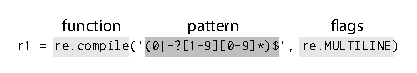
\includegraphics[width=\columnwidth]{featureUse/illustrations/exampleUsage.eps}
\vspace{-12pt}
\caption{Example of one regex utilization}
\vspace{-6pt}
\label{fig:exampleUsage}
\end{figure}

\noindent \textbf{Pattern}: A \emph{pattern} is extracted from a utilization, as shown in Figure~\ref{fig:exampleUsage}. In essence, it is a string, but more formally it is an ordered series of regular expression language feature tokens.  The pattern in Figure~\ref{fig:exampleUsage}  will match if it finds a zero at the end of a line, or a (possibly negative) integer at the end of a line (i.e., due to the {\tt -?} sequence denoting zero or one instance of the {\tt -}).

Note that because the vast majority of regex features are shared across most general programming languages (e.g., Java, C, C\#, or Ruby), a Python {pattern} will (almost always) behave the same when used in other languages, whereas a utilization is not universal in the same way (i.e., it may not compile in other languages, even with small modifications to function and flag names).
As an example, the {\tt re.MULTILINE} flag, or similar, is present in Python, Java, and C\#, but  the Python {\tt re.DOTALL} flag is not present in C\# though it has an equivalent flag in Java.

In this work, we primarily focus on patterns since they are cross-cutting across languages and are the primary way of specifying the matching behavior. Next, we describe the research questions, data set collection and analysis.

\subsection{Research Questions}
\label{sec:rqs}
To understand the contexts in which regexes are used  and feature usage, we perform a survey of developers and explore regular expressions found in Python projects on GitHub. We aim to answer the following research questions:\\

\noindent \textbf{RQ1:} In what contexts do professional developers use regular expressions?

We designed and deployed a survey about when, why, and how often they use regular expressions. This was completed by 18 professional developers at a small software company.\\

\noindent \textbf{RQ2:} How  is the {\tt re} module used in Python projects?

We explore invocations of  the {\tt re} module in \DTLfetch{data}{key}{nProjScanned}{value} Python projects scraped from GitHub.\\


\noindent \textbf{RQ3:} Which regular expression language features are most commonly used in Python?

We consider regex language features to be tokens that specify the matching behavior of a regex pattern, for example,  the {\tt +} in {\tt ab+}.  All studied features are listed and described in Table~\ref{table:featureStats} with examples. We then map the feature coverage for four common regex support tools, brics, hampi, RE2 and Rex, and explore survey responses regarding feature usage for some of the less supported features.\\

\noindent \textbf{RQ4:} How behaviorally similar are regexes across projects?

As this is a first step in understanding behavioral overlap in
regexes, we measure similarity between pairs of regexes by overlap in matching strings. For each regex, matching strings are generated and then  evaluated against each other regex to compute pairwise similarity. Then we use clustering to form behaviorally similar groupings.


%\noindent \textbf{RQ5:} What is the impact of \emph{not} supporting various regular expression features on tool users and designers?
%
%We use semantic analysis to illustrate the impact of missing features on a tool's applicability by identifying what each feature (or group of features) is commonly used for. \\

%Next, we describe our survey, how the corpus of regex patterns was built, how features were analyzed, and how the clustering was performed.

\subsection{Survey Design and Implementation}
\label{study:survey}
To understand the context of when and how programmers use regular expressions,
we designed a survey, implemented using Google Forms, with 40 questions. The questions asked about regex usage frequency, languages, purposes, pain points, and the use of various language
features.\footnote{survey link removed for anonymity}%\url{https://github.com/softwarekitty/tour_de_source/blob/master/regex_usage_in_practice_survey.pdf}}
Participation was voluntary and participants were entered in a lottery for a \$50 gift card.

Our goal was to understand the practices of professional developers. Thus, we deployed the survey to 22 professional developers at Dwolla, a small software company that provides tools for online and mobile payment management. While this sample comes from a single company, we note anecdotally that Dwolla is a start-up and most of the developers worked previously for other software companies, and thus bring their past experiences with them. Surveyed developers have nine years of experience, on average, indicating the results may generalize beyond a single, small software company, but further study is needed.


%The questions asked about regex usage frequency, languages, purposes, and the use of various language features, as explored in Section~\ref{rq1:survey} and Section~\ref{results:rq3}.
%\todoMid{More details on survey design}


\subsection{Regex Corpus}
\label{study:corpus}
Our goal was to collect regexes from a variety of projects to represent the breadth of how developers use the language features.
Using the GitHub API, we scraped \DTLfetch{data}{key}{nProjScanned}{value}  projects containing Python code.
We did so  by dividing a range of about 8 million repo IDs
into 32 sections of equal size and scanning  for Python projects from the beginning of those
segments until we ran out of memory. At that point, we felt we had enough data
to do an analysis without further perfecting our mining techniques. We built
the AST of each Python file in each project to find utilizations of the {\tt re} module
functions. In most projects, almost all regex utilizations are present in the
most recent version of a project, but to be more thorough, we also scanned up
to 19 earlier versions. The number 20 was chosen to try and maximize returns on
computing resources invested after observing the scanning process in many hours
of trial scans.
% If the project had fewer than 20 commits, then all commits were scanned.
% The most recent commit was always included, and the spacing between all other chosen commits was determined by dividing the remaining number of commits by 19 (rounding as needed).
All regex utilizations were obtained, sans duplicates. Within a project, a duplicate utilization was marked when two versions of the same file have the same function, pattern and flags.  In the end, we observed and recorded \DTLfetch{data}{key}{nUsages}{value} non-duplicate regex utilizations in \DTLfetch{data}{key}{nProjScanned}{value} projects.

In collecting the set of distinct patterns for analysis,  we ignore the \DTLfetch{data}{key}{percentBadFlags}{value}\%  of utilizations using flags, which can alter regex behavior.  An additional \DTLfetch{data}{key}{percentInvalidPattern}{value}\% of utilizations contained patterns that could not be compiled because the pattern was non-static (e.g., used some runtime variable).
The remaining \DTLfetch{data}{key}{percentCleanUsages}{value}\% (\DTLfetch{data}{key}{nCleanUsages}{value}) of the utilizations were collapsed into \DTLfetch{data}{key}{nDistinctPatterns}{value} distinct pattern strings.  Each of the pattern strings was pre-processed by removing Python quotes (\verb!`\\W!' becomes \verb!\\W!), unescaping escaped characters (\verb!\\W! becomes \verb!\W!) and parsing the resulting  string using an ANTLR-based, open source PCRE parser\footnote{\url{https://github.com/bkiers/pcre-parser}}.
This parser was unable to support \DTLfetch{data}{key}{percentUnicode}{value}\% (\DTLfetch{data}{key}{N_UNICODE}{value}) of the patterns due to unsupported unicode characters.  Another \DTLfetch{data}{key}{percentAlien}{value}\% (\DTLfetch{data}{key}{N_ALIEN}{value}) of the patterns used regex features that we  chose to exclude because they appeared very rarely (e.g., reference conditions).  An additional 0.1\% (16) of the patterns were excluded because they were empty or otherwise malformed so as to cause a parsing error.

The \DTLfetch{data}{key}{nCorpus}{value} distinct pattern strings that remain were each assigned a weight value equal to the number of distinct projects the pattern appeared in.  We  refer to this set of weighted, distinct pattern strings as the \emph{corpus}.

\subsection{Analyzing Features}
\label{study:features}
For each escaped pattern, the PCRE-parser produces a tree of feature tokens, which is converted to a vector by counting the number of each token  in the tree.  For a simple example, consider the patterns in Figure~\ref{fig:featureParsing}.  The pattern \verb!`^m+(f(z)*)+'! contains four different types of tokens. It has the kleene star (KLE), which is specified using the asterisk \verb!`*'! character, additional repetition (ADD), which is specified using the plus \verb!`+'! character, capture groups (CG), which are specified using pairs of parenthesis \verb!`(...)'! characters, and the start anchor (STR), which is specified using the caret \verb!`^'! character at the beginning of a pattern. A list of all features and abbreviations is provided in Table~\ref{table:featureStats}.

\begin{figure}[tb]
\centering
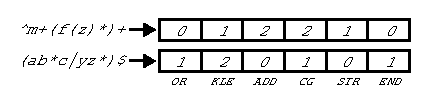
\includegraphics[height=0.6in]{featureUse/illustrations/featureParsing.eps}
\caption{Two patterns parsed into feature vectors}
\label{fig:featureParsing}
\vspace{-12pt}
\end{figure}

Once all patterns were transformed into vectors, we examined each feature independently for all patterns, tracking the number of patterns and  projects that the each feature appears in at least once.




\subsection{Clustering and Behavioral Similarity}
An ideal analysis of regex behavioral similarity would use subsumption or containment analysis. However, we struggled to find a tool that could facilitate such an analysis. Further, regular expressions in code libraries (e.g., for Python, Java) are not the same as regular languages in formal language theory. Some features of regular expression libraries, such as backreferences, make the libraries more expressive than regular languages. This allows a regular expression pattern to match, for example, repeat words, such as ``cabcab", using the pattern {\tt ([a-z]+)\verb!\!1}. However, building an automaton to recognize such a pattern and to facilitate containment analysis, is infeasible.
For these reasons, we developed a similarity analysis based on string matching.


\begin{figure}[tb]
\centering

\includegraphics[height=0.6in]{featureUse/illustrations/minimalMatrix.eps}
\caption{A similarity matrix created by counting strings matched}
\label{fig:minimalMatrix}
\end{figure}


\begin{figure}[tb]
\centering
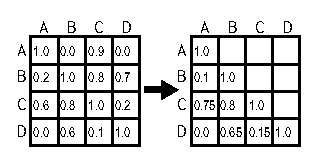
\includegraphics[width=0.7\columnwidth]{featureUse/illustrations/matrixToGraph.eps}
\vspace{-6pt}
\caption{Creating a similarity graph from a similarity matrix}
\vspace{-6pt}
\label{fig:matrixToGraph}
\end{figure}

Our similarity analysis clusters regular expressions by their behavioral similarity on matched strings.
Consider two unspecified patterns {\tt A} and {\tt B}, a set {\tt mA} of 100 strings that pattern {\tt A} matches, and a set {\tt mB} of 100 strings that pattern {\tt B} matches.
If pattern {\tt B} matches 90 of the 100 strings in the set {\tt mA}, then {\tt B} is 90\% similar to {\tt A}.
If pattern {\tt A} only matches 50 of the strings in {\tt mB}, then {\tt A} is 50\% similar to {\tt B}.
We use similarity scores to create a similarity matrix as shown in Figure~\ref{fig:minimalMatrix}.
In row {\tt A}, column {\tt B} we see that {\tt B} is 90\% similar to {\tt A}.
In row {\tt B}, column {\tt A}, we see that {\tt A} is 50\% similar to {\tt B}.  Each pattern is always 100\% similar to itself, by definition.

Once the similarity matrix is built, the values of cells reflected across the diagonal of the matrix are averaged to create a half-matrix of undirected similarity edges, as illustrated in Figure~\ref{fig:matrixToGraph}.
This facilitates clustering using the  Markov Clustering (MCL) algorithm\footnote{\url{http://micans.org/mcl/}}.
We chose MCL  because it offers a fast and tunable way to cluster items by similarity and it is particularly useful when the number of clusters is not known \emph{a priori}.


In the implementation, strings are generated for each pattern using Rex~\cite{rex}.  Rex generates matching strings by representing the regular expression as an automaton, and then passing that automation to a constraint solver that generates members for it\footnote{\url{http://research.microsoft.com/en-us/projects/rex/}}.  If the regex matches a finite set of strings smaller than 400, Rex will produce a list of all possible strings.
Our goal is to generate 400 strings for each pattern to balance the runtime of the similarity analysis with the precision of the similarity calculations.


For clustering, we prune the similarity matrix to retain all similarity values greater than or equal to 0.75, setting the rest to zero, and then using MCL.
This threshold was selected based on recommendations in the MCL manual. The impact of lowering the threshold would likely result  in either the same number of more diverse clusters, or a larger number of clusters, but is unlikely to markedly change the largest clusters or their summaries, which are the focus of our analysis for RQ4 (Section~\ref{rq4:results}), but further study is needed to substantiate this claim.
We also note that MCL can also be tuned using many parameters, including inflation and filtering out all but the top-k edges for each node.
After exploring the quality of the clusters using various tuning parameter combinations, the best clusters (by inspection) were found using an inflation value of 1.8 and k=83.   The top 100 clusters are categorized by inspection into six categories of behavior. % (see Section~\ref{rq4:results}).

The end result is clusters and categories of highly behaviorally similar regular expressions, though we note that this approach has a tendency to over-approximate the similarity of two regexes. We measure similarity based on a finite set of generated strings, but some regexes  match an infinite set (e.g., \verb!ab*c!), so measuring similarity based on the first 400 strings may lead to an artificially high similarity value. To mitigate this threat, we chose a large number of generated strings for each regex, but future work includes exploring other approaches to computing regex similarity.


%\todoNow{fix this before the ICSE deadline - after putting several days into this, I have a partial fix but the fact is there was information loss when going between the java program and the cs program and back again.  So it remains to be seen if it will be feasible to do non-automatic repairs.}
%
%
%We note that there was an operational error in pulling patterns from our database prior to the similarity analysis and clustering, so that 224 patterns (2.3\%) of the 9,727 patterns were omitted. These were duplicate patterns that were quoted differently (for example \verb!`\W'! and \verb!"\W"!).  The result of this error is a slight underestimate in number of projects per pattern (and per cluster), and a slight over-estimate in the pattern, file and project statistics shown in Table~\ref{table:featureStats}.  We do not believe that this error affects our conclusions.



\section{Results}
\label{sec:results}



Next, we present the results of each research question.

\subsection{RQ1: How do developers use regexes?}
\label{rq1:survey}
The survey was completed by 18 participants (82\% response rate) that identified as software developer/maintainers.
Respondents have an average of nine years of programming experience ($\sigma = 4.28$).
On average, survey participants report to compose 172 regexes per year ($\sigma$ = 250) and compose regexes on average once per month, with 28\% composing multiple regexes in a week and an additional 22\% composing regexes once per week. That is, 50\% of respondents uses regexes at least weekly.
Table~\ref{tab:regexenviron} shows how frequently participants compose regexes using each of several languages and technical environments.
Six (33\%) of the survey participants report to compose regexes using general purpose programming languages (e.g., Java, C, C\#) 1-5 times per year and five (28\%) do this 6-10 times per year.  For command line usage in tools such as grep, 6 (33\%) participants use regexes 51+ times per year. Yet, regexes were rarely used in query languages like SQL. Upon further investigation, it turns out the surveyed developers were not on teams that dealt heavily with a database.



%\newcommand{\horiz}{\hspace{2.1pt}}

\begin{table}[t]
\caption{Survey results for number of regexes composed per year by technical environment (RQ1) \label{tab:regexenviron}}
\begin{center}
\begin{small}
\begin{tabular}{l | r @{  \horiz} r @{ \horiz } r @{ \horiz } r @{ \horiz } r @{ \horiz } r }
\toprule
\textbf{Language/Environment} & 0 & 1-5 & 6-10 & 11-20 & 21-50 & 51+ \\  \hline \bigstrut
General  (e.g., Java)  & 1 & 6 & 5 & 3& 1& 2 \\ \hline \bigstrut
Scripting  (e.g., Perl) &5 &4 &3 &3 &2  &1 \\ \hline \bigstrut
Query  (e.g., SQL) & 15&2 &0 &0 &1  & 0\\ \hline \bigstrut
Command line (e.g., grep)   &2 &5 &3 &2 &0  &6 \\ \hline \bigstrut
Text editor (e.g., IntelliJ)   & 2& 5& 0& 5& 1& 5\\
\bottomrule
\end{tabular}
\end{small}
\end{center}
\vspace{-12pt}
\end{table}

\begin{table}
\caption{Survey results for regex usage frequencies for  activities, averaged using a 6-point likert scale: Very Frequently=6, Frequently=5, Occasionally=4, Rarely=3, Very Rarely=2, and Never=1 (RQ1)\label{tab:regexactivities}}
\begin{center}
\begin{small}
\begin{tabular}{l|c}
\toprule
\textbf{Activity} & \textbf{Frequency} \\  \hline \bigstrut
Locating content within a file or files & 4.4\\ \hline \bigstrut
Capturing parts of strings & 4.3 \\ \hline \bigstrut
Parsing user input & 4.0\\ \hline \bigstrut
Counting lines that match a pattern & 3.2\\ \hline \bigstrut
Counting  substrings that match a pattern & 3.2\\  \hline \bigstrut
Parsing generated text & 3.0\\  \hline \bigstrut
Filtering collections (lists, tables, etc.) & 3.0 \\ \hline \bigstrut
Checking for a single character & 1.7\\
\bottomrule
\end{tabular}
\end{small}
\end{center}
\vspace{-12pt}
\end{table}

Table~\ref{tab:regexactivities} shows how frequently, on average, the participants use
regexes for various activities.
Participants answered questions using a 6-point likert scale including very frequently~(6), frequently~(5), occasionally~(4), rarely~(3), very rarely~(2), and never~(1).
%Assigning values from 1 to 6, where 6 is the most frequent, the responses were averaged across participants.
Averaging across participants, among the most common usages are capturing parts of a string and locating content within a file, with both occurring somewhere between occasionally and frequently.

Using a similar 7-point likert scale that includes `always' as a seventh point, developers indicated that they test their regexes with the same frequency as they test their code (average response was 5.2, which is between frequently and very frequently).  Half of the  developers indicate that they use external tools to test their regexes, and the other half indicated that they only use tests that they write themselves. Of the nine developers using tools, six mentioned online composition aides such as \url{regex101.com} where a regex and input string are entered, and the input string is highlighted according to what is matched.
%The other three developers mentioned 'ScalaCheck' (a testing framework), 'IDE regex plugins', and 'Language specific Regexlib'.

When asked an open ended question about pain points encountered with regular expressions, we observed three main categories. The most common, ``hard to compose," was represented in 61\% (11) responses. Next,
 39\% (7) developers responded that regexes are ``hard to read" and 17\% (3) indicated difficulties with ``inconsistency across implementations," which manifest when using regexes in multiple languages. These responses do not sum to 18 as three developers provided multiple parts in their answers.

\vspace{6pt}
\textbf{Summary - RQ1:}
%The survey validates the assumption that regex are widely used by professional software developers and sheds some light into the context in which regexes are used.
%Future research into regex can focus on activities that prove to be most important to developers, namely capturing parts of strings and searching for specific content.
%Although research into regex use in general purpose and scripting languages is important, usage within command line tools and text editors should also be considered.
Common uses of regexes include locating content within a file, capturing parts of strings, and parsing user input.
The fact that all the surveyed developers compose regexes, and half of the developers use tools to test their regexes indicates the importance of tool development for regex.  Developers complain about regexes being hard to read and hard to write.%, and most of the tools that they indicate using are (suitably) focused on composition.

\begin{table}[tb]
\begin{center}
\begin{small}
\caption{How saturated are projects with utilizations? (RQ2)}
\label{table:saturation}

\begin{tabular}{l|ccccc}
\toprule
source & Q1 & Avg & Med & Q3 & Max \\ 
 \hline \bigstrut
utilizations per project & 2 & 32 & 5 & 19 & 1,427 \\ 
 \hline \bigstrut
files per project & 2 & 53 & 6 & 21 & 5,963 \\ 
 \hline \bigstrut
utilizing files per project & 1 & 11 & 2 & 6 & 541 \\ 
 \hline \bigstrut
utilizations per file & 1 & 2 & 1 & 3 & 207 \\ 
\bottomrule
\end{tabular}
\end{small}
\end{center}
\vspace{-12pt}
\end{table}


\subsection{RQ2: How  is the {\tt re} module used?}
We explore regex utilizations and flags used in the scraped Python projects.
Out of the \DTLfetch{data}{key}{nProjScanned}{value}\ projects scanned, \DTLfetch{data}{key}{percentProjectsUsingRegex}{value}\% (\DTLfetch{data}{key}{nProjectsUsingRegex}{value}) contained at least one regex utilization.  To illustrate how saturated projects are with regexes, we measure utilizations per project, files scanned per project, files contained utilizations, and  utilizations  per file, as shown in Table~\ref{table:saturation}.

Of projects containing at least one utilization, the average utilizations per project was 32 and the maximum  was 1,427.  The project with the most utilizations is a C\# project\footnote{\url{https://github.com/Ouroboros/Arianrhod}} that maintains a collection of source code for 20 Python libraries, including larger libraries like {\tt pip}, {\tt celery} and {\tt ipython}.  These larger Python libraries contain many utilizations.
From Table~\ref{table:saturation}, we also see that each project had an average of 11 files containing any utilization, and each of these files had an average of 2 utilizations.



% \begin{figure}[tb]
% \centering
% 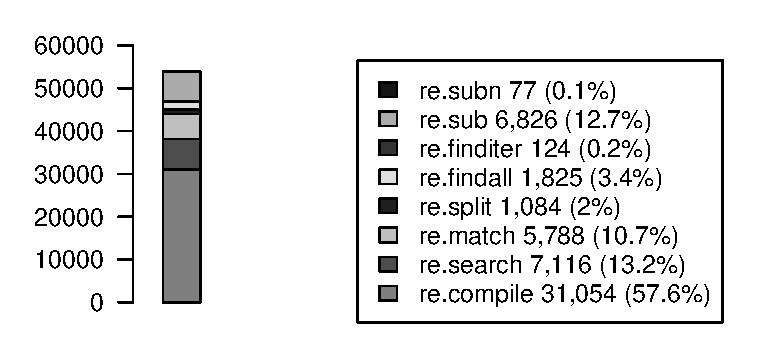
\includegraphics[width=\columnwidth]{featureUse/analysis_output/partFunctions.eps}
% \vspace{-12pt}
% \caption{How often are  {\tt re} functions used? (RQ2)}
% \vspace{-6pt}
% \label{fig:partFunctions}
% \end{figure}

%\begin{figure}[tb]
%\centering
%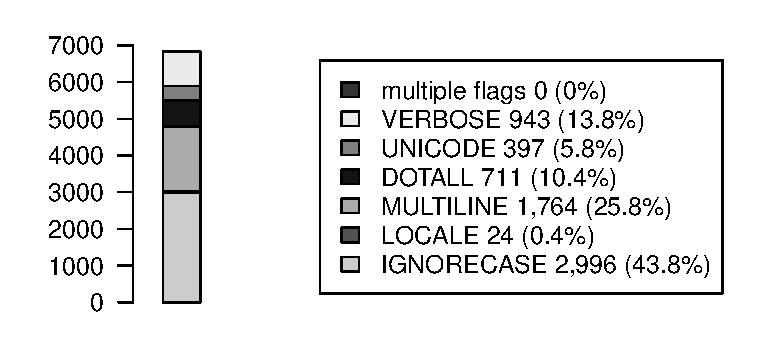
\includegraphics[width=0.9\columnwidth]{../analysis_output/partFlags.eps}
%\vspace{-6pt}
%\caption{Which behavioral flags are used? (RQ2)}
%\vspace{-6pt}
%\label{fig:partFlags}
%\end{figure}

\begin{table*}[h!tb]
\begin{center}
\begin{small}
\caption{How frequently do features appear in projects? (RQ3)}
\label{table:featureStats}
\begin{tabular}{ll@{ }llc @{ } c @{ }c @{ } c  cccccc @{}}
rank & code & description & example & brics & hampi & Rex & RE2 & nPatterns & \% patterns & nProjects & \% projects \\ 
\toprule[0.16em]
1 & ADD & one-or-more repetition & \begin{minipage}{0.5in}\begin{verbatim}z+\end{verbatim}\end{minipage} & \yes & \yes & \yes & \yes & 6,003 & 44.1 & 1,204 & 73.2 \\ 
\midrule
2 & CG & a capture group & \begin{minipage}{0.5in}\begin{verbatim}(caught)\end{verbatim}\end{minipage} & \yes & \yes & \yes & \yes & 7,130 & 52.4 & 1,194 & 72.6 \\ 
\midrule
3 & KLE & zero-or-more repetition & \begin{minipage}{0.5in}\begin{verbatim}.*\end{verbatim}\end{minipage} & \yes & \yes & \yes & \yes & 6,017 & 44.3 & 1,099 & 66.8 \\ 
\midrule
4 & CCC & custom character class & \begin{minipage}{0.5in}\begin{verbatim}[aeiou]\end{verbatim}\end{minipage} & \yes & \yes & \yes & \yes & 4,468 & 32.9 & 1,026 & 62.4 \\ 
\midrule
5 & ANY & any non-newline char & \begin{minipage}{0.5in}\begin{verbatim}.\end{verbatim}\end{minipage} & \yes & \yes & \yes & \yes & 4,657 & 34.3 & 1,005 & 61.1 \\ 
\midrule
6 & RNG & chars within a range & \begin{minipage}{0.5in}\begin{verbatim}[a-z]\end{verbatim}\end{minipage} & \yes & \yes & \yes & \yes & 2,631 & 19.3 & 848 & 51.6 \\ 
\midrule
7 & STR & start-of-line & \begin{minipage}{0.5in}\begin{verbatim}^\end{verbatim}\end{minipage} & \no & \yes & \yes & \yes & 3,563 & 26.2 & 846 & 51.4 \\ 
\midrule
8 & END & end-of-line & \begin{minipage}{0.5in}\begin{verbatim}$\end{verbatim}\end{minipage} & \no & \yes & \yes & \yes & 3,169 & 23.3 & 827 & 50.3 \\ 
\midrule[0.12em]
9 & NCCC & negated CCC & \begin{minipage}{0.5in}\begin{verbatim}[^qwxf]\end{verbatim}\end{minipage} & \yes & \yes & \yes & \yes & 1,935 & 14.2 & 776 & 47.2 \\ 
\midrule
10 & WSP & \textbackslash t \textbackslash n \textbackslash r \textbackslash v \textbackslash f or space & \begin{minipage}{0.5in}\begin{verbatim}\s\end{verbatim}\end{minipage} & \no & \yes & \yes & \yes & 2,846 & 20.9 & 762 & 46.3 \\ 
\midrule
11 & OR & logical or & \begin{minipage}{0.5in}\begin{verbatim}a|b\end{verbatim}\end{minipage} & \yes & \yes & \yes & \yes & 2,102 & 15.5 & 708 & 43 \\ 
\midrule
12 & DEC & any of: 0123456789 & \begin{minipage}{0.5in}\begin{verbatim}\d\end{verbatim}\end{minipage} & \no & \yes & \yes & \yes & 2,297 & 16.9 & 692 & 42.1 \\ 
\midrule
13 & WRD & [a-zA-Z0-9\_] & \begin{minipage}{0.5in}\begin{verbatim}\w\end{verbatim}\end{minipage} & \no & \yes & \yes & \yes & 1,430 & 10.5 & 650 & 39.5 \\ 
\midrule
14 & QST & zero-or-one repetition & \begin{minipage}{0.5in}\begin{verbatim}z?\end{verbatim}\end{minipage} & \yes & \yes & \yes & \yes & 1,871 & 13.8 & 645 & 39.2 \\ 
\midrule
15 & LZY & as few reps as possible & \begin{minipage}{0.5in}\begin{verbatim}z+?\end{verbatim}\end{minipage} & \no & \yes & \no & \yes & 1,300 & 9.6 & 605 & 36.8 \\ 
\midrule
16 & NCG & group without capturing & \begin{minipage}{0.5in}\begin{verbatim}a(?:b)c\end{verbatim}\end{minipage} & \no & \yes & \no & \yes & 791 & 5.8 & 404 & 24.6 \\ 
\midrule
17 & PNG & named capture group & \begin{minipage}{0.5in}\begin{verbatim}(?P<name>x)\end{verbatim}\end{minipage} & \no & \yes & \no & \yes & 915 & 6.7 & 354 & 21.5 \\ 
\midrule
18 & SNG & exactly n repetition & \begin{minipage}{0.5in}\begin{verbatim}z{8}\end{verbatim}\end{minipage} & \yes & \yes & \yes & \yes & 581 & 4.3 & 340 & 20.7 \\ 
\midrule
19 & NWSP & any non-whitespace & \begin{minipage}{0.5in}\begin{verbatim}\S\end{verbatim}\end{minipage} & \no & \yes & \yes & \yes & 484 & 3.6 & 270 & 16.4 \\ 
\midrule
20 & DBB & $n\le x \le m$ repetition & \begin{minipage}{0.5in}\begin{verbatim}z{3,8}\end{verbatim}\end{minipage} & \yes & \yes & \yes & \yes & 367 & 2.7 & 238 & 14.5 \\ 
\midrule
21 & NLKA & sequence doesn't follow  & \begin{minipage}{0.5in}\begin{verbatim}a(?!yz)\end{verbatim}\end{minipage} & \no & \no & \no & \no & 131 & 1 & 183 & 11.1 \\ 
\midrule
22 & WNW & word/non-word boundary & \begin{minipage}{0.5in}\begin{verbatim}\b\end{verbatim}\end{minipage} & \no & \no & \no & \yes & 248 & 1.8 & 166 & 10.1 \\ 
\midrule
23 & NWRD & non-word chars & \begin{minipage}{0.5in}\begin{verbatim}\W\end{verbatim}\end{minipage} & \no & \yes & \yes & \yes & 94 & 0.7 & 165 & 10 \\ 
\midrule
24 & LWB & at least n repetition & \begin{minipage}{0.5in}\begin{verbatim}z{15,}\end{verbatim}\end{minipage} & \yes & \yes & \yes & \yes & 91 & 0.7 & 158 & 9.6 \\ 
\midrule
25 & LKA & matching sequence follows & \begin{minipage}{0.5in}\begin{verbatim}a(?=bc)\end{verbatim}\end{minipage} & \no & \no & \no & \no & 112 & 0.8 & 158 & 9.6 \\ 
\midrule
26 & OPT & options wrapper & \begin{minipage}{0.5in}\begin{verbatim}(?i)CasE\end{verbatim}\end{minipage} & \no & \yes & \no & \yes & 231 & 1.7 & 154 & 9.4 \\ 
\midrule
27 & NLKB & sequence doesn't precede & \begin{minipage}{0.5in}\begin{verbatim}(?<!x)yz\end{verbatim}\end{minipage} & \no & \no & \no & \no & 94 & 0.7 & 137 & 8.3 \\ 
\midrule[0.12em]
28 & LKB & matching sequence precedes & \begin{minipage}{0.5in}\begin{verbatim}(?<=a)bc\end{verbatim}\end{minipage} & \no & \no & \no & \no & 80 & 0.6 & 120 & 7.3 \\ 
\midrule
29 & ENDZ & absolute end of string & \begin{minipage}{0.5in}\begin{verbatim}\Z\end{verbatim}\end{minipage} & \no & \no & \no & \yes & 89 & 0.7 & 90 & 5.5 \\ 
\midrule
30 & BKR & match the $i^{th}$ CG & \begin{minipage}{0.5in}\begin{verbatim}\1\end{verbatim}\end{minipage} & \no & \no & \no & \no & 60 & 0.4 & 84 & 5.1 \\ 
\midrule
31 & NDEC & any non-decimal & \begin{minipage}{0.5in}\begin{verbatim}\D\end{verbatim}\end{minipage} & \no & \yes & \yes & \yes & 36 & 0.3 & 58 & 3.5 \\ 
\midrule
32 & BKRN & references PNG & \begin{minipage}{0.5in}\begin{verbatim}\g<name>\end{verbatim}\end{minipage} & \no & \yes & \no & \no & 17 & 0.1 & 28 & 1.7 \\ 
\midrule
33 & VWSP & matches U+000B & \begin{minipage}{0.5in}\begin{verbatim}\v\end{verbatim}\end{minipage} & \no & \no & \yes & \yes & 13 & 0.1 & 15 & 0.9 \\ 
\midrule
34 & NWNW & negated WNW & \begin{minipage}{0.5in}\begin{verbatim}\B\end{verbatim}\end{minipage} & \no & \no & \no & \yes & 4 & 0 & 11 & 0.7 \\ 
\bottomrule[0.13em]
\end{tabular}
\end{small}
\end{center}
\vspace{-12pt}
\end{table*}


The number of projects that use each of the {\tt re} functions is shown in Figure~\ref{fig:partFunctions}.  The y-axis denotes the total utilizations, with a maximum of \DTLfetch{data}{key}{nUsages}{value}. The {\tt re.compile} function encompasses \DTLfetch{data}{key}{percentCompile}{value}\% of all utilizations. %, presumably because each usage of the other seven functions can accept a regex object compiled using {\tt re.compile} as an argument.
Note that compiled objects can also be used to call functions of the re module, ie {\tt compiledObject.findall(...)}, but we ignore these utilizations so that our analysis is easier to automate, and because we are primarily interested in extracting the patterns which these 8 functions contain.


%When considering flag use, we excluded the default flag, which is built into the {\tt re} module, and present internally whenever no flag is used.
Of all utilizations, \DTLfetch{data}{key}{percentFlags0}{value}\% had no flag, or explicitly specified the default flag.  The debug flag, which causes the {\tt re} regex engine to display extra information about its parsing, was never observed. This may be because developers use it for debugging and choose not to commit it to their repositories.
% Figure~\ref{fig:partFlags} presents the number of projects in which each flag appears. Ignorecase (\DTLfetch{data}{key}{percentI}{value}\%) and multiline (\DTLfetch{data}{key}{percentM}{value}\%) were the most frequently used.   Although multiple flags can be combined using a bitwise or, this was never observed.

\vspace{6pt}
\textbf{Summary - RQ2:}
Only about half of the Python projects sampled contained any utilizations.  Most utilizations used the {\tt re.compile} function to compile a regex object before actually using the regex to find a match.  Most utilizations did not use a flag to modify matching behavior.




%The most frequently observed patterns were used to match whitespace and digits.

\subsection{RQ3: Regex language feature usage}
\label{results:rq3}

We  count the usages of each feature per project and as compared to all distinct regex patterns in the corpus.



\subsubsection{Feature Usage}
\label{sec:featureUsage}
Table~\ref{table:featureStats} displays feature usage from the corpus and relates it to four major regex related projects. Only features appearing in at least 10 projects are listed.
The first column, \emph{rank}, lists the rank of a feature (relative to other features) in terms of the number of projects in which it appears. The next column, \emph{code}, gives a succinct reference string for the feature, and is followed by a \emph{description} column that provides a brief comment on what the feature does.  The \emph{example} column provides a short example of how the feature can be used.
% For example, the most common feature observed in the corpus is \emph{one-or-more repetition}, which is specified in a pattern by using the {\tt +} character in conjunction with some sub-pattern that should repeat one or more times.  The code for this feature is \emph{ADD}, and the short example provided is \verb!z+!.
The next four columns, (i.e., \emph{brics}, \emph{hampi}, \emph{Rex}, and \emph{RE2}), map to the four major research projects chosen for our investigation (see Section~\ref{regextoolsresults}).  We indicate that a project supports a feature with the `\yes' symbol, and indicate that a project does not support the feature with the `\no' symbol.
The final four columns contain two pairs of usage statistics.  The first pair contains the number and percent of \emph{patterns} that a feature appears in, out of the 13,597 patterns that make up the corpus.  The second pair of columns contain the number and percent of \emph{projects} that a feature appears in out of the 1,645 projects scanned that contain at least one utilization.

One notable omission from Table~\ref{table:featureStats} is the literal feature, which is used  to specify matching any specific character.  An example pattern that contains only one literal token is the pattern \verb!`a'!.  This pattern only matches the lowercase letter `a'.  The literal feature was found in \DTLfetch{data}{key}{P_LITERAL_PRESENT}{value}\% of patterns.
%, and accounted for \DTLfetch{data}{key}{P_LITERAL_TOKENS}{value}\% of all tokens.
We consider the literal feature to be necessary for any regex related tool to support, and so exclude it from Table~\ref{table:featureStats} and the rest of the feature analysis.



The eight most commonly used features, ADD, CG, KLE, CCC, ANY, RNG, STR and END,
appear in over half the projects. %The remaining 26 features appear in less than half of the projects containing utilizations.
CG is more commonly used in patterns than the highest ranked feature (ADD) by a wide margin (over 8\%), even though they appear in similar numbers of projects.

\subsubsection{Feature Support in Regex Tools}
\label{regextoolsresults}
While there are many regex tools available, in this work, we focus on the feature support for  four tools, brics, hampi, Rex and RE2, which offer diversity across developers (i.e., Microsoft, Google, open source, and academia) and applications. Further, as we wanted to perform a feature analysis, these four tools and their features are well-documented, allowing for easy comparison.

% We  mapped the features from the corpus to those features supported by the four regular expression engines described in Section~\ref{sec:related}: brics, hampi, RE2, and Rex.
To create the tool mappings, we consulted documentation for each tool. For brics, we collected the set of supported features using the formal grammar\footnote{\url{http://www.brics.dk/automaton/doc/index.html?dk/brics/automaton/RegExp.html}}.  For hampi, we manually inspected the set of regexes included in the {\tt lib/regex-hampi/sampleRegex} file within the hampi repository\footnote{\url{https://code.google.com/p/hampi/downloads/list}} (this may have been an overestimation, as this included more features than specified by the formal grammar\footnote{\url{http://people.csail.mit.edu/akiezun/hampi/Grammar.html}}).  For RE2, we used the  supported feature documentation\footnote{\url{https://re2.googlecode.com/hg/doc/syntax.html}}.  For Rex, we collected the feature set empirically because we tried to parse all scraped patterns with Rex for the behavioral analysis (Section~\ref{rq4:results}), and Rex provides comprehensive error feedback for unsupported features.

%\todoLast{Were there any features supported by the tools that we did not find in the corpus? Answer: RE2 has a lot of features we didn't study and that weren't found in the corpus in any substantial quantity.  I think this is addressed by the earlier mention: Only features appearing in at least 10 projects are listed.}


Of the four projects selected for this analysis, RE2 supports the most studied features (28 features) followed by hampi (25 features),  Rex (21 features), and brics (12 features).  All projects support the 8 most commonly used features except brics, which does not support STR or END.
%All projects support NCC, OR, and the four less common repetition features: QST, SNG, DBB and LWB.  RE2 is the only project to support the WNW, ENDZ and NWNW features.
No projects support the four look-around features LKA, NLKA, LKB and NLKB.  RE2 and hampi support the LZY, NCG, PNG and OPT features, whereas brics and Rex do not.%, which inspired in part the survey questions about feature usage.


\subsubsection{Survey Results for Feature Usage}
The pattern language for Python, which is used to compose regexes, supports default character classes like the ANY or dot character class: \verb!.! meaning, `any character except newline'. % (a full list of features and examples is in the first four columns of Table~\ref{table:featureStats}).
It also supports three other default character classes: \verb!\d!, \verb!\w!, \verb!\s! (and their negations). All of these default character classes can be simulated using the custom character class (CCC) feature, which can create semantically equivalent regexes.
For example  the decimal character class: \verb!\d! is equivalent to a CCC containing all 10 digits:  \verb!\d! $\equiv$ \verb![0123456789]! $\equiv$ \verb![0-9]!.
%Users have a choice when using regex between writing \verb!\d! and \verb![0-9]! and whereas the first option may be shorter, the second may seem more intuitive and readable.
Other default character classes such as the word character class: \verb!\w! may not be as intuitive to encode in a CCC: \verb![a-zA-Z0-9_]!.

Survey participants were asked if they use only CCC, use CCC more than default, use both equally, use default more than CCC or use only default.  Results for this question are shown in Table~\ref{tab:cccvsdefault}, with 67\% (12) indicating that they use default the most.
%Participants were also asked to explain their preferences.
 Participants who favored CCC indicated that ``it is more explicit," whereas the participants who favored default character classes said,  ``it is less verbose" and ``I like using built-in code."



\begin{table}
\caption{Survey results for preferences between custom character and default character classes (RQ3) \label{tab:cccvsdefault}}
\begin{center}
\begin{small}
\begin{tabular}{l|c}
\toprule
\textbf{Preference} & \textbf{Frequency} \\  \hline \bigstrut
use only CCC & 1\\ \hline \bigstrut
use CCC more than default & 5 \\ \hline \bigstrut
use both equally & 2\\ \hline \bigstrut
use default more than CCC & 10\\ \hline \bigstrut
use only default & 2\\
\bottomrule
\end{tabular}
\end{small}
\end{center}
\vspace{-12pt}
\end{table}

To further explore how participants use various regex features, participants were asked five questions about how frequently they use specific related groups of features,
%\begin{itemize} \itemsep -2pt
%    \item endpoint anchors (STR, END): \verb!^! and \verb!$!
%    \item capture groups(CG): (capture me)
%    \item word boundaries (WNW): \verb!word\b!
%    \item (negative) look-ahead/behinds (LKA, NLKA, LKB, NLKB): \verb!a(?=bc)!, \verb!(?<!x)yz!, \verb!(?<=a)!, \verb!a(?!yz)!
%    \item lazy repetition (LZY): \verb!ab+?!, \verb!xy{2,3}?!
%\end{itemize}
%These features were
chosen based on the tool feature support explored in Section~\ref{regextoolsresults}.
Results are shown in Table~\ref{tab:regexfeaturegroups}, indicating that lazy repetition and look-ahead features are rarely used and capture groups and endpoint anchors are occasionally to frequently used.


\begin{table}
\caption{Survey results for regex usage frequencies, averaged using a 6-point likert scale: Very Frequently=6, Frequently=5, Occasionally=4, Rarely=3, Very Rarely=2, and Never=1 (RQ3) \label{tab:regexfeaturegroups}}
\begin{center}
\begin{small}
\begin{tabular}{llc}
\toprule
\textbf{Group} & \textbf{Code} &  \textbf{Frequency} \\  \hline \bigstrut
endpoint anchors & (STR, END) & 4.4\\ \hline \bigstrut
capture groups & (CG) & 4.2 \\ \hline \bigstrut
word boundaries & (WNW) & 3.5 \\ \hline \bigstrut
lazy repetition & (LZY) &  2.9\\ \hline \bigstrut
\multirow{2}{*}{(neg) look-ahead/behind} &  (LKA, NLKA,  & \multirow{2}{*}{2.5}\\
& LKB, NLKB) & \\
\bottomrule
\end{tabular}
\end{small}
\end{center}
\vspace{-12pt}
\end{table}



\vspace{6pt}
\textbf{Summary - RQ3:}
The eight most common features are found in over 50\% of the projects.
%, with two of those not being supported by brics.
%We identify RE2 as the project supporting the most features.%, and identify groups of features supported or not supported by the four regex projects.
%I was confused by the 'at least occasionally' verbage, at first it looked like 'the least occasionally'
Shown in Table~\ref{table:featureStats}, the STR and END features are present in over half of the scanned projects containing utilizations.  In our survey, over half (56\%) of the respondents answered that they use endpoint anchors frequently or very frequently, and none of them claimed to never use them.
%The brics library does not support this feature, which is a missed opportunity for developers who could otherwise have used brics to model their regexes that use STR and END.

The LZY feature  is present in over 36\% of scanned projects with utilizations, and yet was not supported by two of the four major regex projects we explored, brics and RE2.
In our developer survey, 11\% (2) of participants use this feature frequently and 6 (33\%) use it occasionally, showing a modest impact on potential users.

%\subsubsection{PNG and BKRN vs CG and BKR}
%The PNG group (python-style named capture groups) and BKRN (back-references: named) are intended to operate together to allow users to name the content that is expected to appear in a capture group.  A simple example of how these can be used together with the named capture group matching some vowel is:
%\verb!(?P<vowel>[aeiou]x(?P=vowel))! which will match the strings 'axa' and 'oxo' but not 'txt'.  The same functionality can be obtained with a much shorter expression: \verb!([aeiou])x\1! where the \verb!'\1'! references the CG started by the first left parenthesis found when moving from left to right.
When survey participants were asked if they prefer to always use numbered (BKR) or named (BKRN) back references, 66\% (12) of survey participants said that they always use BKR, and the remaining 33\% (6) said ``it depends."  No participants preferred named capture groups.  BKR is present in 5\% of scanned projects, while BKRN is present in only 1.7\%, which corroborates our findings that numbered  are generally preferred over named capture groups.

\subsection{RQ4: Regex behavioral similarity}
\label{rq4:results}


In clustering the regular expressions, we are most interested in observing behavior of regexes found in multiple projects.  Starting with the 13,597 patterns of the corpus, we discarded 10,015 (74\%) patterns that were not found in multiple projects.
Then we excluded an additional 711 (5\%) patterns that contain features not supported by Rex.  We studied the remaining 2,871 (21\%) patterns using our similarity analysis technique. The impact is that 923 projects were excluded from the data set for the similarity analysis. Omitted features are indicated in Table~\ref{table:featureStats} for Rex.
%The generated strings for each pattern are used to measure the pairwise similarity for all patterns and construct the similarity matrix.


%\subsubsection{Rationale for Behavioral Clustering}


%\subsubsection{General Information About Clusters Found}
From 2,871 distinct patterns, MCL clustering identified 186 clusters with 2 or more patterns, and 2,042 clusters of size 1.
%Recall that only pairs of patterns with a similarity level of 0.75 were included in the matrix passed to MCL.
 The average size of clusters larger than size one was 4.5.  Each pattern belongs to exactly one cluster.

%\subsubsection{An Example Cluster}

%Three example strings generated by Rex for the first pattern are: `-()', `*'8(5)', `Oe()'.  For the third pattern, Rex generated these three strings: ` ()', `(q)F', `(n)M'.  The pattern: \verb!\(.*\)$! is very similar, but will not match the string `(n)M', and so was placed in a different cluster.

\begin{table}
\begin{center}
\caption{Sample from an example cluster (RQ4)}
\label{table:exampleCluster}
\begin{small}
\begin{tabular}
{lcc | lcc}
\toprule
index & pattern & nProjects & index & pattern & nProjects \\
 \hline \bigstrut
1 & \begin{minipage}{0.3in}\begin{verbatim}`:+'\end{verbatim}\end{minipage} & 8 & 5 & \begin{minipage}{0.5in}\begin{verbatim}`[:]'\end{verbatim}\end{minipage} & 6 \\
 \hline \bigstrut
2 & \begin{minipage}{0.3in}\begin{verbatim}`(:)'\end{verbatim}\end{minipage} & 8 & 6 & \begin{minipage}{0.6in}\begin{verbatim}`([^:]+):(.*)'\end{verbatim}\end{minipage} & 6 \\
 \hline \bigstrut
3 & \begin{minipage}{0.3in}\begin{verbatim}`(:+)'\end{verbatim}\end{minipage} & 8 & 7 & \begin{minipage}{0.5in}\begin{verbatim}`\s*:\s*'\end{verbatim}\end{minipage} & 4 \\
 \hline \bigstrut
4 & \begin{minipage}{0.3in}\begin{verbatim}`(:)(:*)'\end{verbatim}\end{minipage} & 8 & 8 & \begin{minipage}{0.5in}\begin{verbatim}`\:'\end{verbatim}\end{minipage} & 2 \\
\bottomrule
\end{tabular}
\vspace{-6pt}
\end{small}
\end{center}
\vspace{-12pt}
\end{table}


%
%\begin{table}
%\begin{center}
%\caption{An example cluster (RQ3)}
%\label{table:exampleCluster}
%\begin{small}
%\begin{tabular}
%{lcc}
%\toprule
%index & pattern & nProjects\\
%\midrule
%1 & \begin{minipage}{0.5in}\begin{verbatim}`\s*,\s*'\end{verbatim}\end{minipage} & 54  \\
%\midrule
%2 & \begin{minipage}{0.5in}\begin{verbatim}`,'\end{verbatim}\end{minipage} & 30 \\
%\midrule
%3 & \begin{minipage}{0.5in}\begin{verbatim}`\s*,'\end{verbatim}\end{minipage} & 16 \\
%\midrule
%4 & \begin{minipage}{0.5in}\begin{verbatim}` ,\s*'\end{verbatim}\end{minipage} & 13 \\
%\midrule
%5 & \begin{minipage}{0.5in}\begin{verbatim}` *, *'\end{verbatim}\end{minipage} & 12 \\
%\midrule
%6 & \begin{minipage}{0.5in}\begin{verbatim}`,\S'\end{verbatim}\end{minipage} & 5 \\
%\midrule
%7 & \begin{minipage}{0.5in}\begin{verbatim}`,.*$'\end{verbatim}\end{minipage} & 3 \\
%\midrule
%8 & \begin{minipage}{0.6in}\begin{verbatim}`(\S+)\s*,\s*'\end{verbatim}\end{minipage} & 2 \\
%\midrule
%9 & \begin{minipage}{0.5in}\begin{verbatim}`,+'\end{verbatim}\end{minipage} & 1 \\
%\midrule
%10 & \begin{minipage}{0.5in}\begin{verbatim}`,\ ?'\end{verbatim}\end{minipage} & 1 \\
%\midrule
%10 & \begin{minipage}{0.5in}\begin{verbatim}`,\s*(\S)'\end{verbatim}\end{minipage} & 1 \\
%\midrule
%11 & \begin{minipage}{0.5in}\begin{verbatim}`\s*(,)\s*'\end{verbatim}\end{minipage} & 1 \\
%\midrule
%12 & \begin{minipage}{0.5in}\begin{verbatim}`\s*\,\s*'\end{verbatim}\end{minipage} & 1 \\
%\bottomrule
%\end{tabular}
%\end{small}
%\end{center}
%\end{table}


%\subsubsection{Using the Smallest Pattern to Represent a Cluster}

Table~\ref{table:exampleCluster} provides an example of a behavioral cluster containing 12 patterns (four longer patterns omitted for brevity). Patterns from this cluster are present in 31 different projects.  All patterns in this cluster share the literal `:' character. The smallest pattern, \verb!`:+'!,  matches one or more colons.


% \begin{figure}[tb]
% \centering
% 
\includegraphics[width=\columnwidth]{../illustrations/clusterEdgesExample.eps}
% \vspace{-12pt}
% \caption{Example Of Similarity Edges Of One Cluster}
% \vspace{-6pt}
% \label{fig:clusterEdgesExample}
% \end{figure}


%Another pattern from this cluster, \verb!([^:]+):(.*)!, requires at least one non-colon character to occur before a colon character.  Our similarity value between these two regexes was below the minimum of 0.75 because Rex generated many strings for `:+' that start with one or more colons.
% Todo: create a graph graphic with edge weights showing similarity values for all 8 of these patterns.
We observe that the smallest pattern in a cluster provides insight about key characteristic that all the patterns in the cluster have in common.  A shorter pattern will tend to have less extraneous behavior because it is specifying less behavior,
yet, in order for the smallest pattern to be clustered, it had to match most of the strings created by Rex from many other patterns within the cluster, and so we observe that {the smallest pattern is useful as a representative of the cluster}.

For the rest of this paper, a cluster will be represented by one of the shortest patterns it contains, followed by the number of projects any member of the cluster appears in, so the cluster in Table~\ref{table:exampleCluster} will be represented as \verb!`:+'(31)!.  This representation is not an attempt to express all notable behavior of patterns within a cluster, but is a useful and meaningful abbreviation.
Other regexes in the cluster may exhibit more diverse behavior, for example the pattern \verb!`([^: ]+):(.*)'! requires a non-colon character to appear before a colon character.

We manually mapped the top 100 largest clusters based on the number of projects into 6 behavioral categories (determined by inspection).  The largest cluster was left out, as it was composed of patterns that trivially matched almost any string, like \verb!`b*'! and \verb!`^'!.  The remaining 99 clusters were all categorized. These clusters are briefly summarized in Table~\ref{tab:clustercats}, showing the name of the category and the number of clusters it represents, patterns in those clusters, and projects. The most common category is \emph{Multi Matches}, which contains clusters that have alternate behaviors (e.g., matching a comma or a semicolon, as in \verb!`,|;'(18)!). Each cluster was mapped to exactly one category. Next, we describe the categories, ordered by the number of projects the regex patterns map to.

%When a cluster can fit in multiple categories, it is placed in the most specific category.  The following six categories are listed in order from most specific behavior to least specific behavior.

\begin{table}
\begin{center}
\begin{small}

\caption{Cluster categories and sizes (RQ4) \label{tab:clustercats}}
\begin{tabular}{lccc}
\toprule
\textbf{Category} & \textbf{Clusters} & \textbf{Patterns} & \textbf{Projects} \\  \hline \bigstrut
Multi Matches & 21 & 237 & 295\\
\hline \bigstrut
Specific Char & 17 & 103 & 184\\
\hline \bigstrut
Anchored Patterns & 20 & 85 & 141\\
\hline \bigstrut
 Content of Parens & 10 & 46 & 111\\
\hline \bigstrut
Two or More Chars & 16 & 40 & 120\\
\hline \bigstrut
Code Search & 15 & 27 & 92 \\
\bottomrule
\end{tabular}
\vspace{-12pt}
\end{small}
\end{center}
\end{table}

%6
\subsubsection{Multiple Matching Alternatives}
The patterns in these clusters match under a variety of conditions by using a character class or a disjunctive \verb!|!.
For example:
\verb!`(\W)'(89)! matches any alphanumeric character, \verb!`(\s)'(89)! matches any whitespace character, \verb!`\d'(58)! matches any numeric character, and \verb!`,|;'(18)! matches a comma or semicolon.  Most of these clusters are represented by patterns that use default character classes, as opposed to custom character classes.  This provides further support for our survey results to the question, \emph{Do you prefer to use custom character classes or default character classes more often?}, in which a majority of participants indicated they use the default classes more than custom.
%This category contains 21 clusters, each appearing in an average of 33 projects.
%Todo: this category is the most general, and has 2 sub-catagories of small CCCs and very large ranges/complex CCCs.
%These clusters have a combined total of 237 patterns, with at least one pattern present in 295 projects.


%5
\subsubsection{Specific Character Must Match}
\label{cluster:single}
Each cluster in this category requires one specific character to match, for example:
\verb!`\n\s*'(42)! matches only if a newline is found, \verb!`:+'(31)! matches only if a colon is found, \verb!`%'(22)!, matches only if a percent sign is found and \verb!`}'(14)! matches only if a right curly brace is found.
Table~\ref{table:exampleCluster} presents a cluster that falls under this category.
% \todoMid{Repair after merge conflict later}
% Table~\ref{table:exampleCluster} presents a cluster that falls under this category. While the cluster is centered on the presence of the \verb!`:'! character, the other regexes in the cluster also exhibit more diverse behavior.
The commonality of this cluster category contrasts with the survey in Section~\ref{rq1:survey} in which participants reported to very rarely or never use regexes to check for a single character (Table~\ref{tab:regexactivities}).
%This category contains 17 clusters, each appearing in an average of 17.1 projects.
% These clusters have a combined total of 103 patterns, with at least one pattern present in 184 projects.

%3
\subsubsection{Anchored Patterns}
Each of the clusters uses at least one endpoint anchor to require matches to be absolutely positioned, for example:
\verb!`(\w+)$'(35)! captures the word characters at the end of the input, \verb!`^\s'(16)! matches a whitespace at the beginning of the input, and \verb!`^-?\d+$'(17)! requires that the entire input is an (optionally negative) integer.
These anchors are the only way in regexes to guarantee that a character does (or does not) appear at a particular location by specifying what is allowed. As an example, \verb!^[-_A-Za-z0-9]+$! says that from beginning to end, only \verb![-_A-Za-z0-9]! characters are allowed, so it will fail to match if undesirable characters, such as \verb!?!, appear anywhere in the string.
%This category contains 20 clusters, each appearing in an average of 15.4 projects.
%These clusters have a combined total of 85 patterns, with at least one pattern present in 141 projects.

%\todoMid{The thing I want to mention about anchored patterns (but have struggled to say in the past) is that they are the only way to guarantee that a character does not appear in a particular location by specifying what is allowed.  Consider the regex }
%\verb!^[-_A-Za-z0-9]+$!
%\todoMid{ which will fail to match if an undesirable character like `?' appears anywhere in the input.  In logic, there is a similar phenomenon.  That is, `Always' is true iff `Not Exists' of the negation is true, and by requiring an entire input to always maintain some abstraction, you can indirectly specify the negation of another (inverse) abstraction.  Even with only one anchor point, a regex like }
%\verb!.*[0-9]$!
%\todoMid{ is creating an ultimatum about the end being a digit.  Without the endpoint anchors, I don't see how one could specify absolutes about an input. }

%2
\subsubsection{Content of Brackets and Parenthesis}
\label{cluster:contentparens}
The clusters in this category center around finding a pair of characters that surround content, often also capturing that content. For example,
\verb!`\(.*\)'(29)! matches when content is surrounded by parentheses and \verb!`".*"'(25)! matches  when content is surrounded by double quotes.  The cluster \verb!`<(.+)>'(23)! matches and captures content surrounded by angled brackets.
%This category contains 10 clusters, each appearing in an average of 18.4 projects.
% These clusters have a combined total of 46 patterns, with at least one pattern present in 111 projects.
%, and \verb!`\[.*\]'(22)! matches when content is surrounded by square brackets
%4
\subsubsection{Two or More Characters in Sequence}
\label{cluster:multiple}
These clusters require several characters in a row to match some pattern, for example:
\verb!`\d+\.\d+'(30)! requires one or more digits followed by a period character, followed by one or more digits.  The cluster \verb!`  '(17)! requires two spaces in a row,
%\verb!`([A-Z][a-z]+[A-Z][^ ]+)'(11)!,
and \verb!`@[a-z]+'(9)! requires the at symbol followed by two or more lowercase characters, as in a twitter handle.
%This category contains 16 clusters, each appearing in an average of 13 projects.
%These clusters have a combined total of 40 patterns, with at least one pattern present in 120 projects.

%\todoMid{Again, it might be interesting to look at what particular sequences are looking like.  I think I mention this again in the discussion, but should we put it here instead?}

%1
\subsubsection{Code Search and Variable Capturing}
\label{cluster:search}
These clusters show a recognizable effort to parse source code or URLs. For example,
\verb!`^https?://'(23)! matches a web address, and \verb!`(.+)=(.+)'(9)! matches an assignment statement, capturing both the variable name and value.
The cluster  \verb!`\$\{([\w\-]+)\}'(11)! matches an evaluated string interpolation and captures the code to evaluate.
%This category contains 15 clusters.%, each appearing in an average of 11.7 projects.
%These clusters have a combined total of 27 patterns, with at least one pattern present in 92 projects.

\vspace{6pt}
\textbf{Summary - RQ4:}
%When tool designers are considering what features to include, data about usage in practice is valuable.  Behavioral similarity clustering  helps to discern these behaviors by looking beyond the structural details of specific patterns and seeing trends in  matching behavior. % We are also able to find out what features are being used in these behavioral trends so that we can make assertions about why certain features are important.
%We used the behavior of individual patterns to form clusters, and identified six main categories for the clusters.
% Overall, we see that many clusters are defined by the presence of particular tokens, such as the colon for the cluster in Table~\ref{table:exampleCluster}.
We identified six main categories that define regex behavior at a high level: matching with alternatives, matching literal characters, matching with sequences, matching with endpoint anchors, parsing contents of brackets or braces, or searching and capturing code. %, and can be considered in conjunction with the self-described regex activities from the survey in Table~\ref{tab:regexactivities} to be representative of common uses for regexes.
%One of the six common cluster categories, \emph{Code Search and Variable Capturing}, has a very specific purpose of parsing source code files. This shows a very specific and common use of regular expressions in practice.




\section{Discussion}
\label{sec:discussion}

In this section, we discuss the implications of these empirical findings
%on tool designers and users of regex tools
 and opportunities for future work.

\subsection{Implications For Tool Designers}
The results have  implications for regex tool designers. % who want to effectively support developers who use regular expressions.

%\subsubsection{All Character Classes Are Common}
%The same character class can be expressed in different ways, for example \verb!`[0-9]'! is equivalent to \verb!`\d'!.  Our results indicate that both approaches are widely used (Table~\ref{tab:cccvsdefault}), so tool builders should continue to support both approaches.


\subsubsection{Finding Specific Content}
Two categorical clusters, \emph{Specific Characters Must Match} (Section~\ref{cluster:single}) and \emph{Two or More Characters in Sequence} (Section~\ref{cluster:multiple}), deal with identifying the presence of specific character(s).
While multiple character matching subsumes single character matching, the overarching theme is that these regexes are looking to validate strings based on the presence of very specific content, as would be done for many common activities listed in Table~\ref{tab:regexactivities}, such as, ``Locating content within a file or files."
%(This is in contract to \emph{capturing} specific content, as \emph{finding} deals with string validation and \emph{capturing} deals with string extraction.)
%As indicated by the clusters of specific character matches in Section~\ref{cluster:single}, finding specific content is important.
%Delimiters that separate items on one line like \verb!`\t'! are also quite common.
%Although survey participants indicated an average frequency of 1.7 (very rarely or never) for ``checking for a single character," we found that 17 of the top 100 clusters revolved around the presence of a single character.
%The commonality of regexes related to finding content is consistent with the top ranked activity for developers, ``Locating content within a file or files."
%and usually this content is located using some small set of characters that the user knows will flag that content.
More study is needed into what content is most frequently searched for, but from our cluster analysis we found that version numbers, twitter or user handles, hex values, decimal numbers, capitalized words, and particular combinations of whitespace, slashes and other delimiters were discernible targets.

%Looking closely at the \emph{Specific Character Must Match} cluster, some of the characters being searched for were \verb!\n!, \verb!-! and \verb!.!, which are all common delimiters in different scenarios. This indicates the need for regex tools to facilitate easy file parsing, or for tools to include built-in support for specific, common types of parsing.


\subsubsection{Capturing Specific Content Near A Delimiter}
The survey results from Section~\ref{rq1:survey} indicate that capturing parts of strings is among the most frequent activities for which developers use regexes.
From a feature perspective, the capture group (CG) is the most frequently used in terms of patterns (Table~\ref{table:featureStats}).  This feature has two functions: 1) logical grouping as would be expected by parenthesis, and 2) retrieval of information in one logical grouping.  As mentioned in Section~\ref{rq4:results}, capturing content was a primary goal evident in several cluster categories.  The fourth-largest category is based entirely on capturing the content between brackets or parentheses (Section~\ref{cluster:contentparens}).

%Combined with the cluster on \emph{Code Search and Variable Capturing} (Section~\ref{cluster:search}), this emphasizes the need for regex tools to  facilitate easy file parsing, or for a tool to include built-in support for specific, common types of parsing.


Many uses of CG also use the ANY and KLE features, eg. \verb!(.*){(.*)}(.*)! and \verb!\\s*([^: ]*)\\s*:(.*)!.  This type of usage frequently revolves around an important delimiter character such as \verb!:! or \verb!\!.  This use case is well supported by existing tools for ASCII characters, but future tools should consider the centrality of this use case and its implications for non-English users of regex tools.  For example, Unicode characters like `U+060D' the Arabic Date Separator, or `U+1806' the Mongolian Todo Soft Hyphen may be used to locate segments of text that a user would want to capture.

%, such as finding a twitter handle (i.e., \verb!@[a-z]+!) or a version number, (i.e., \verb!v[0-9]+.*!).
%and then capture specific content, such as the actual twitter handle or the actual version number, but may not know how to do that capture groups and may rely on string parsing instead.

%\todoMid{The main difference between the Specific Character Must Match group and the multiple characters must match is that the first can subsume the second.  I think it's important to defend this and expose that we understand that our simplification of clusters to their shortest representative combined with the behavioral clustering technique will drastically over-emphasize similarities revolving around single characters, so instead of listing this as a major group, or a major finding, we may need to admit that it is an emphasis that our technique introduces artificially.  I think that in practice, the patterns being searched for usually revolve around more than just a single character, although maybe not a lot more than that.  I think it is more telling that despite our technique's tendency to over-cluster things around a single character, there was still an entire category that required two or more characters, and so those specific pairs or triples or whatever in that cluster are extremely key character combinations.  Let's see a few of those that seem to make sense: }
%\verb! {2,}!
%\todoMid{ :two or more spaces, }
%\verb!@[a-z]+!
%\todoMid{ :a lowercase twitter handle or similar,}
% \verb!\\$[()]!
% \todoMid{ :a dollar followed by either paren, }
% \verb!v[0-9]+.*!
% \todoMid{ :the letter `v' followed by some numbers, perhaps a version number.  }

\subsubsection{Counting Lines}
Text files containing one unit of information per line are common in a wide variety of applications (for example .log and .csv files).  Out of the 13,597 patterns in the corpus, 3,410 (25\%) contained ANY followed by KLE  (i.e., \verb!`.*'!), often at the end of the pattern.
One reasonable explanation for this tendency to put \verb!`.*'! at the end of a pattern is that users want to disregard all matches after the first match on a single line in order to count how many distinct lines the match occurs on.  Survey participants indicated an average frequency of ``Counting lines that match a pattern" and ``Counting substrings that match a pattern" at 3.2 or rarely/occasionally. It may be valuable for tool builders to include support for common activities such as line counting.



%\todoMid{In a completely unrelated train of thought, I have been considering how regexes are one major way, and perhaps the only practical way in the world of computer science to handle the invisible characters like ASCII 0-32.  That's 33 characters like `backspace' and `end of medium' and 'vertical tab' that can appear in text and cause problems.  I've heard them called `Gremlins'.  So what do people do?  They write regexes to clean those out.}



\subsection{Opportunities For Future Work}

There are many opportunities for future work. %\todoLast{Hey Kids! Need a thesis topic? Here's a bunch! Promote this awesome section earlier}




\subsubsection{Refactoring Regexes}
The survey showed that users want readability and find the lack of readable regexes to be a major pain point.
This provides an opportunity to introduce refactoring transformations to enhance readability or comprehension.
As one opportunity, certain character classes are logically equivalent and can be expressed differently, for example, \verb!\d! $\equiv$ \verb![0123456789]! $\equiv$ \verb![0-9]!. While \verb!\d! is more succinct, \verb![0-9]! may be easier to read, so a refactoring for \emph{default to custom character classes} could be introduced.
Human studies are needed to evaluate the readability and comprehension of various regex features in order to define and support appropriate regex refactorings.

Another avenue of refactoring could be for performance. Various implementations of regex libraries may perform more efficiently with some features than others. An evaluation of regex feature implementation speeds would facilitate semantic transformations based on performance, similar to performance refactorings for LabVIEW~\cite{chambers2013smell, chambers2015impact}.


Additionally, some developers may  \emph{find} specific content with a regex  and then subsequently \emph{capture} it with string parsing, which may be more error prone than using a capture group and indicates a missed opportunity to use the full extent of regex libraries. Future work will explore source code to identify the frequency of such occurrences and design refactorings to better utilize regex library features.

%Other similar refactoring techniques may become evident with a more thorough search.  A tool that preserved the exact behavior of a regex but optimized for readability could be incorporated into an IDE and relieve some developer pain.  More research is needed into why certain character classes are considered more readable, as has been done for other refactoring work (e.g.,~\cite{StoleeTSE2013}).
%Similarly, there are several principals that can be followed to enhance the performance of a regex.  Using non-capture groups whenever possible, avoiding backtracking, etc.  In theory it seems possible to build a compiler that could compose a regex with identical behavior but with better readability and performance.

\vspace{-2pt}
\subsubsection{Migration  Support for Developers}
Within standard programming languages, regular expressions libraries are very common, yet there are subtle  differences between language libraries in the supported features. For example, Java supports possessive quantifiers like \verb! `ab*+c'! (here the `+' is modifying the `*' to make it possessive) whereas Python does not. Differences among programming language implementations was identified as a pain point for using regular expressions by 17\% of the survey participants. This provides a future opportunity for tools that translate between regex utilizations in various languages.

\vspace{-2pt}
\subsubsection{Similarity Beyond String Matching}
There are various ways to compute similarity between regexes, each with different tradeoffs.
While the similarity analysis we employ over-approximates similarity when compared to containment analysis, it may under-approximate similarity in another sense.
%We define behavioral similarity based on strings matched by pairs of regular expressions. However, t
For example, two regexes that have dissimilar matching behavior could be very similar in purpose and in the eyes of the developer. For example, \verb!commit:\[(\d+)\] - (.*)! and \verb!push:\[(\d+)\] - (.*)! could both be used to  capture the id and command from a versioning system, but match very different sets of strings. Future work would apply abstractions to the regex strings, such as removing or relaxing literals, prior to similarity analysis to capture and cluster such similarities.

From another perspective, our regex similarity measure, and even containment analysis, could treat behaviorally identical regexes as the same, when  their usage in practice is completely different. For example, in Table~\ref{table:exampleCluster}, the regexes \verb!`:+'! and \verb!`(:+)'! are behaviorally identical in that they match the same strings, except the latter uses a capture group. In practice, these may be used very differently, where the former may be used for validation and the latter for extraction. This usage difference could be observed by code  analysis, and is left for future work.

\vspace{-2pt}
\subsubsection{Automated Regex Repair}
Regular expression errors are common and have produced thousands of bug reports~\cite{Spishak:2012:TSR:2318202.2318207}. This provides an opportunity to introduce automated repair techniques for regular expressions.
Recent approaches to automated program repair rely on mutation operators to make small changes to source code and then re-run the test suite (e.g., ~\cite{cacm10, genprog-tse-journal}). In regular expressions, it is likely that the broken regex is close, semantically, to the desired regex. Syntax changes through mutation operators could lead to big changes in behavior, so we hypothesize that using the semantic clusters identified in Section~\ref{rq4:results} to identify potential repair candidates could efficiently and effectively converge on a repair candidate.

\subsubsection{Developer Awareness of Best Practices}
One category of clusters, \emph{Content of Brackets and Parenthesis}, parses the contents of angle brackets, which may indicate developers are using regexes to parse HTML or XML.  As the contents of angle brackets are usually unconstrained, regexes are a poor replacement for XML or HTML parsers.  This may be a missed opportunity for the regex users to take advantage of more robust tools. More research is needed into how regex users discover best practices and how aware they are of how regexes should and should not be used.
%http://english.stackexchange.com/questions/50851/the-contents-are-or-the-contents-is

%\subsubsection{Support for Regexes Composition}
%According to our survey, over 60\% of developers find regexes to be difficult to compose. Additionally, developers frequently or very frequently write tests for their regexes. This provides an opportunity to instead





\subsubsection{Tool-Specific Regex Exploration}
In some environments, such as command line or text editor, regexes are used extensively by the surveyed developers (Section~\ref{rq1:survey}), but these regular expressions do not persist. Thus, using a repository analysis for feature usage only illustrates part of how regexes are used in practice. Exploring how the feature usage differs between environments would help inform tool developers about how to best support regex usage in context, and is left for future work.


% \subsubsection{A Modern WRD Character Class}
% \todoMid{update}
% One unexpected result of our clustering is that, behaviorally speaking, the negation of the word class NWRD was used in 208 projects, while the word class itself was used in only 114 projects. After inspecting several projects using the patterns found in this behavioral cluster, we concluded that most users are trying to sanitize arbitrary strings that must conform to a system character set requirement, such as requirements for filenames.  For example, a user might replace all NWRD matching characters with the `\_' to guarantee that an arbitrary string can be used as a filename.  We also considered the largest cluster using custom character classes (\verb?`[^ -~]'(122)?) and concluded that users are constructing a more permissive version of the NWRD character class, to allow more non-letter, non-digit characters than just the `\_' in their sanitized strings.  More research is needed to determine if a more modern WRD class could be useful, and if so, what characters set is preferred.




\section{Threats to Validity}
\label{sec:threats}
The following threats impact our results and conclusions:

%\subsection{Conclusion}
\textbf{Reliability of Measures:} The validity of our survey results is dependent on the clarity of the questions. The authors went through several iterations of the survey and included examples for all the regex feature descriptions to improve understandability.

The similarity measure between regexes used in the cluster algorithm is computed empirically rather than analytically, and the more Rex-generated strings used to compute the similarity measure, the more likely it is to be accurate. Our experiments used 400 strings to balance performance and precision, but a higher number could lead to more cohesive clusters. Additionally, regex patters that use any feature not supported by Rex were omitted from the cluster analysis. Last, the threshold of 0.75 was chosen based on the MCL recommendation, but it may not create optimal clusters. %\todoMid{talk about tools for formal analysis}
%In our clustering algorithm, we require a similarity level of 0.75 so that we do not over-estimate the similarity between regular  expressions.\todoNow{what does this last sentence mean?  Is this paragraph okay?}

%\subsection{Internal}

\textbf{Instrumentation:} Regular expression patterns were clustered using strings generated by the Rex tool.  We assume that the strings generated by Rex are reasonably diverse to help characterize the regex behavior. To mitigate this threat, Rex generated 400 strings per regex and we inspected strings randomly to ensure diversity.

Implementation errors are a risk for research involving repository analysis. To combat this, we have tested our code and made the repository publicly available\footnote{GitHub link removed for anonymity}.%\url{https://github.com/softwarekitty/tour_de_source}}.

\textbf{Selection:} We mined \DTLfetch{data}{key}{nProjScanned}{value} Python projects from GitHub, which is  small compared to all available projects with Python code. The projects were mined using the GitHub API which sorts the projects by creation date. By using the API, the goal was to reduce  sampling bias from the researchers.

We also did not scrape all commits in every project for regular expression utilizations, rather, we grabbed each project every 20 commits. It is possible that in between the scanned commits, a regex utilization was added and then removed, leading to fewer utilizations in our final data set.

\textbf{Recall bias:} Survey participants were asked to reflect on their past behavior, which may not  represent actual behavior. To mitigate this, we designed the survey to lead participants to think about their behavior before summarizing (e.g., asking how often they use regexes in each of several environments before asking about usage frequency).

%\subsection{Construct}

%\textbf{Hypothesis guessing:} The lead author was an employee of Dwolla when the survey was run, so participant behavior may have been affected by their relationship with the author. To combat this, the beginning of the survey stated, ``As this is for research, please answer as accurately as possible, not guessing what is the desired answer and providing that."

%\subsection{External}

\textbf{Interaction of Selection and Treatment:} Our survey participants were software developers from a small startup company and may not be representative of developers who use regexes. Given that the average participant has nine years of development experience, their responses likely pull from a variety of experiences with regular expression usage, but replication with a more diverse set of developers is needed.

\textbf{Interaction of Setting and Treatment:}
We only explore regular expressions in Python projects so these results may be coupled with the activities performed using Python and not generalize to other languages. The regex usage context reported by survey participants, however, includes information on  regex usage in a  variety of settings and languages. Future work will replicate this study in other languages.



%The survey results are from a set of developers at one company and may not generalize to other developers at that company or at other companies. While the results provide some information on regex usage, repeating the survey to a larger set of diverse developers will increase the generalizeability of the results.
%%
%
%In extracting patterns for analysis, we omit utilizations that contain flags since flags provide refinements on the functionality of the pattern as it is used in the project. Given that only 12.7\% of all utilizations used flags, the impact on the clusters should be minimal.
%
%%The feature analysis is dependent on the features identified in the PCRE parser.
%


%\vspace{-6pt}
\section{Conclusion}
\label{sec:conclusion}
In this work, we have explored the contexts in which regular expressions are used as well as the features and behavioral similarities of regexes found in open source Python projects. In a survey of 18 professional developers, we find that 50\% compose regular expressions at least weekly. The most common purposes are locating content within a file or capturing parts of strings. The most difficult parts about working with regular expressions were reported to be composing and reading them.
In a study of regular expression usage in nearly 4,000 Python projects, we find that over 42\% of projects contain a regular expression.
We present an approach to measure behavioral similarity between regexes by generating strings that match one regex and pairwise  testing the remaining regexes against it. This similarity measure is used to form cross-project behavioral clusters. In the top 100 largest clusters, we find that capturing the contents of brackets,  searching for delimiter characters and matching alternative values were common behaviors.
These results have implications for tool designers and for future research aimed at better supporting developers in using regular expressions.


% use section* for acknowledgement
%\vspace{-6pt}
\section*{Acknowledgment}
%\vspace{-2pt}
Special thanks to the Dwolla developers for their survey participation.
This work is supported in part by NSF SHF-1218265, NSF SHF-EAGER-1446932, and the Harpole-Pentair endowment at Iowa State University.

%\vspace{12pt}
\newpage
\bibliographystyle{abbrv}

% The bibliography should be embedded for final submission.
\balance
\bibliography{biblio}



% that's all folks
%\end{document}

